% \documentclass{article}
% \usepackage[top=1.25in, bottom=1.1in, left=1.25in, right=1in]{geometry}
% \usepackage[utf8]{inputenc}
% \usepackage{fullpage}
% \usepackage {setspace}
% \usepackage[hang,flushmargin]{footmisc} %control footnote indent
% \usepackage{url} % for website links
% \usepackage{amssymb,amsmath}%for matrix
% \usepackage{graphicx}%for figure
% \usepackage{appendix}%for appendix
% \usepackage{float}
% \usepackage{multirow}
% \usepackage{longtable}
% \usepackage{morefloats}%in case there are too many float tables and figures
% \usepackage{caption}
% \usepackage{subcaption}
% \usepackage{listings}
% \captionsetup[subtable]{font=normal}
% \usepackage{color}
% \usepackage{hyperref}
% \usepackage[round]{natbib}

% %\usepackage{Sweave}
% \setlength{\parindent}{0em}
% \setlength{\parskip}{0.5em}


% \graphicspath{{0.plots/}}



% \begin{document}


\subsection{Introduction}
Joint models (JM) of longitudinal and time-to-event data have been well developed in the literature as they are highly applicable in the setting of longitudinal data analysis with event-related terminal events (e.g., dropout or death which is related to the longitudinal process), or for survival analysis with a time dependent covariate measured with error \citep{self1992modeling, tsiatis1995modeling}. JM have been extensively studied in recent years and an excellent review is provided by \cite{tsiatis2004joint}. % quantile regression and its advantages over mean regression
Within the traditional JM framework, a linear mixed model (LMM) sub-model is used to model the longitudinal continuous outcome. To account for within-subject correlation, measurements from the same subject share the random effects, and random errors are assumed to be normally distributed \citep{laird1982random}. However, if normality assumption of the random errors is violated (even after applying various outcome transformations), an LMM is not appropriate. Further, an LMM  models covariate effects on the conditional mean of the longitudinal outcome. However, in many clinical studies it is of interest to make inference or prediction on median, lower or higher quantiles of the longitudinal outcome. For example, in a study of the impact of various health factors on low birth weight, which is closely associated with infant mortality and development of chronic diseases, researchers fit a quantile regression (QR) model and find several significantly different covariate effects on lower birth weight compared with that on the mean birth weight \citep{koenker2001quantile}. Thus, QR may serve as an alternative to conditional mean regression when the aforementioned limitations are present, or when the subject matter dictates.

In contrast to mean regression such as LMM, original QR models offer a flexible framework that relaxes the distributional assumption, and provides a way to study covariate effects on various quantiles of the outcome \citep{koenker2005quantile}. QR has attracted much attention since the seminal work of \cite{koenker1978regression}, and extensions for longitudinal data have been explored by many authors, i.e., \cite{koenker2004quantile}, \cite{geraci2007quantile}, \cite{geraci2013linear}, and \cite{kozumi2011gibbs}. To our knowledge, \cite{farcomeni2015longitudinal} first incorporated a linear quantile mixed model (LQMM) into a JM for longitudinal and survival processes, for which they utilized a Monte Carlo Expectation Maximization (MCEM) algorithm for parameter estimation.

Our work is motivated by the Neurobiological Predictors of Huntington's Disease (HD) study (PREDICT-HD; ClinicalTrials.gov number NCT00051324), a prospective observational study (n=1078) designed to detect early neurobiological predictors of HD. A total of 40 longitudinal biomarkers were measured during the study follow-up of 12 years, where the outcome of interest was time to motor diagnosis of HD (referred to as HD onset). As the primary focus of this study was to measure the association between longitudinal biomarkers and risk of HD onset, the clinical question lends itself to a joint modeling approach. The left panel of Figure~\ref{fig:data_neurotot} displays the scatter plot and kernel density (on the right side) of total motor score (TMS), a commonly used rating criteria of body motion abilities based on the Unified Huntington Disease Rating Scale (UHDRS). The left panel suggests that TMS increases (deteriorates) as time progresses. The right panel of Figure~\ref{fig:data_neurotot} displays the mean TMS values over time for subjects with follow-up time less than 48 months (solid red line), 48$-$72 months (dotted green line), and more than 72 months (slashed blue line). It indicates that subjects with shorter follow-up tend to have higher TMS values (worse mobility). Because subjects with higher TMS are at greater risk of developing HD, it is of particular interest to explore the disease progression in a higher TMS subpopulation as opposed to modeling the conditional mean of TMS. Similar plots for other biomarkers are presented in Section~\ref{sec:data}.

\begin{figure}[H]
\centering
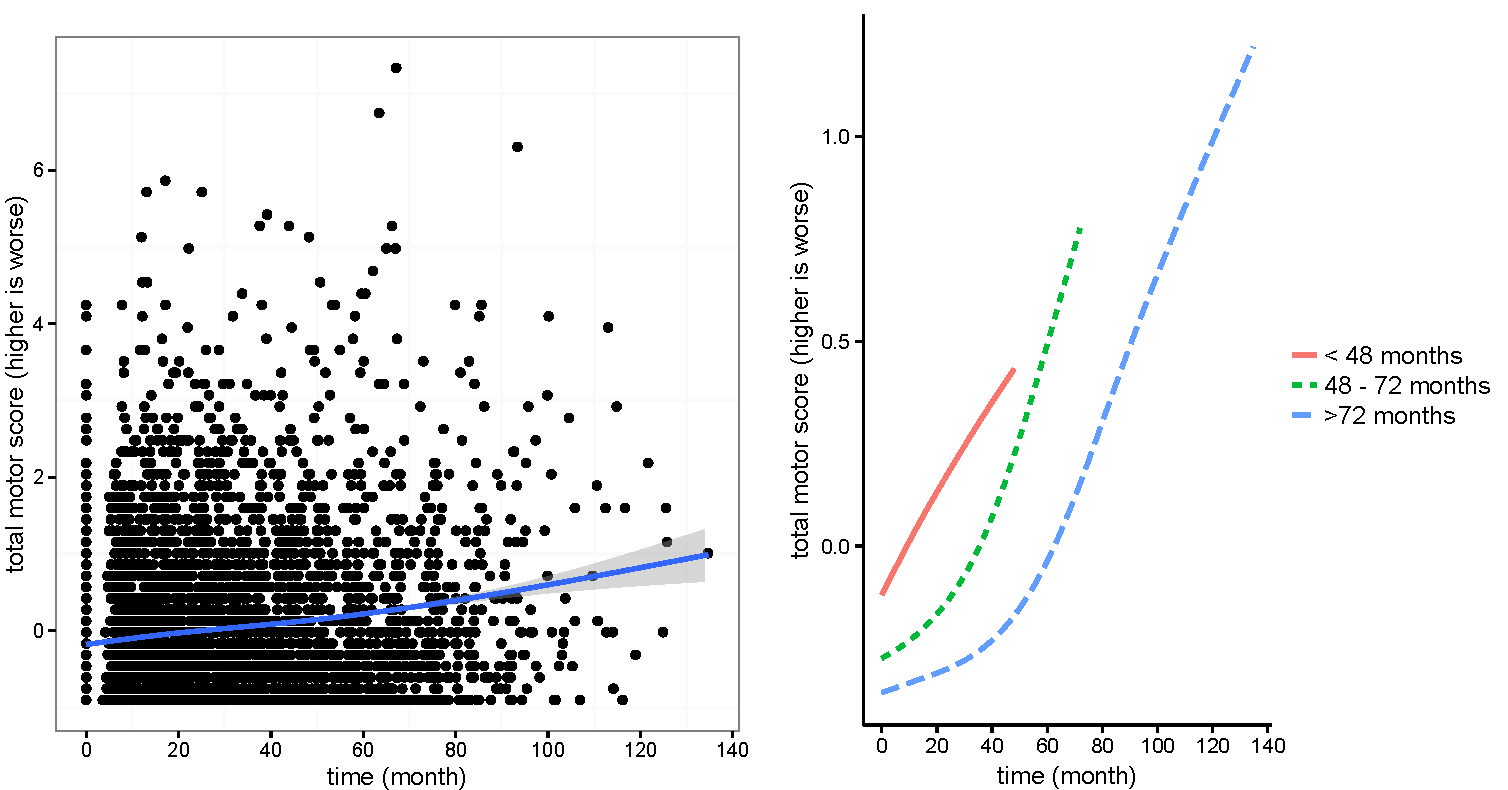
\includegraphics[width=\columnwidth]{TMS_scatter_loess_grp.pdf}
\caption{Left panel: Scatter plot (with loess curve) and kernel density plot (right side) for {total motor score} from the study population (time unit: month; lower total motor score is better); right panel: Mean total motor score values over time.}
\label{fig:data_neurotot}
\end{figure}

Moreover, we are specifically interested in estimating the risk of developing HD for those study participants who are still free of the disease. The JM framework offers a novel way of making such personalized dynamic predictions of future event-free probability \citep{rizopoulos2011dynamic,taylor2013real}. A key feature of these dynamic predictions frameworks is that the predictive measures can be dynamically updated as additional longitudinal measurements become available for the target subjects, providing instantaneous risk assessment. In order to make dynamic predictions in the LQMM-based JM framework, we develop a fully Bayesian algorithm for model estimation and dynamic predictions under the new quantile regression joint models (QRJM) framework. The algorithm consists of two parts. First, we build the QRJM framework consisting of an LQMM for the longitudinal process and a proportional hazard model (PHM) for the time to HD onset process and then draw Bayesian inference, based on a large study population. Second, we make predictions of future HD-free probability for a subject using his or her longitudinal biomarker trajectory information. To estimate the risk of a future event, we explore the posterior distribution of the fixed effects and the predictions of the subject-specific random effects from our QRJM. Moreover, we dynamically update the predictions as long as an individual is free of HD and new longitudinal measurements can be obtained. {Our work is different from \cite{farcomeni2015longitudinal} in the following: (1) we consider a fully Bayesian QRJM for statistical inference while \cite{farcomeni2015longitudinal} used a MCEM algorithm; (2) more importantly, by taking advantage of the posterior distributions of model parameters and subject-specif random effects, we develop a dynamic predictions procedure for future event-free probability under the proposed QRJM.}

The rest of this article proceeds as follows. In Section~\ref{sec:methods}, we give details of the QRJM and statistical methods used for inference and dynamic predictions. In Section~\ref{sec:simulation}, we present two simulation studies to validate the proposed methods. In Section~\ref{sec:data}, we apply the proposed methods to the motivating data set. We conclude the article with a discussion in Section~\ref{sec:discussion}.

% \bibliographystyle{plainnat}%%%%%%%%%%%%%%%%%%%%
% \addcontentsline{toc}{section}{References}
% \bibliography{QRJM}
% \end{document}

